%% ****** Start of file template.aps ****** %
%%
%%
%%   This file is part of the APS files in the REVTeX 4 distribution.
%%   Version 4.0 of REVTeX, August 2001
%%
%%
%%   Copyright (c) 2001 The American Physical Society.
%%
%%   See the REVTeX 4 README file for restrictions and more information.
%%
%
% This is a template for producing manuscripts for use with REVTEX 4.0
% Copy this file to another name and then work on that file.
% That way, you always have this original template file to use.
%
% Group addresses by affiliation; use superscriptaddress for long
% author lists, or if there are many overlapping affiliations.
% For Phys. Rev. appearance, change preprint to twocolumn.
% Choose pra, prb, prc, prd, pre, prl, prstab, or rmp for journal
%  Add 'draft' option to mark overfull boxes with black boxes
%  Add 'showpacs' option to make PACS codes appear
%  Add 'showkeys' option to make keywords appear
\documentclass{revtex4}
%\documentclass[aps,prl,preprint,superscriptaddress]{revtex4}
%\documentclass[aps,prl,twocolumn,groupedaddress]{revtex4}
\usepackage[dvipdf]{graphicx}
\usepackage{appendix}
%\usepackage{dcolumn}

% You should use BibTeX and apsrev.bst for references
% Choosing a journal automatically selects the correct APS
% BibTeX style file (bst file), so only uncomment the line
% below if necessary.
%\bibliographystyle{apsrev}

\begin{document}

% Use the \preprint command to place your local institutional report
% number in the upper righthand corner of the title page in preprint mode.
% Multiple \preprint commands are allowed.
% Use the 'preprintnumbers' class option to override journal defaults
% to display numbers if necessary
%\preprint{}

%Title of paper
\title{Measurements of the Electromagnetic Force Constants}

% repeat the \author .. \affiliation  etc. as needed
% \email, \thanks, \homepage, \altaffiliation all apply to the current
% author. Explanatory text should go in the []'s, actual e-mail
% address or url should go in the {}'s for \email and \homepage.
% Please use the appropriate macro foreach each type of information

% \affiliation command applies to all authors since the last
% \affiliation command. The \affiliation command should follow the
% other information
% \affiliation can be followed by \email, \homepage, \thanks as well.
%\author{Jason P. Longacre}
%\homepage[]{Your web page}
%\thanks{}
%\altaffiliation{}
\author{Physics 2502, University of Connecticut}
%\author{R.T. Jones}
%\affiliation{University of Connecticut}

%Collaboration name if desired (requires use of superscriptaddress
%option in \documentclass). \noaffiliation is required (may also be
%used with the \author command).
%\collaboration can be followed by \email, \homepage, \thanks as well.
%\collaboration{}
%\noaffiliation

\date{\today}

\begin{abstract}
There are two fundamental constants in the classical theory of
electromagnetism, called the permittivity and the permeability of
free space.  These constants determine the magnitude of the electric
and magnetic forces that exist between charges and between currents in
a vacuum.  Students measure the values of these two constants in this
experiment, using a balance to compare electromagnetic forces between
charged plates and current-carrying wires to the gravitational force
on small masses.  The product of these two constants is related to the
speed of light, so this experiment can also be considered as a measurement
of the speed of light.  The measurements are carried out in air, so the
speed of light being measured is that in the medium of air.
\end{abstract}

% insert suggested PACS numbers in braces on next line
%\pacs{}
% insert suggested keywords - APS authors don't need to do this
%\keywords{}

\setlength{\topmargin}{0in}

%\maketitle must follow title, authors, abstract, \pacs, and \keywords
\maketitle

% body of paper here - Use proper section commands
% References should be done using the \cite, \ref, and \label commands

%% The normal text is displayed in two-column format, but special
%% sections spanning both columns can be inserted within the page
%% format so that long equations can be displayed. Use
%% sparingly.
%%\begin{widetext}
%% put long equation here
%%\end{widetext}
%
%% figures should be put into the text as floats.
%% Use the graphics or graphicx packages (distributed with LaTeX2e)
%% and the \includegraphics macro defined in those packages.
%% See the LaTeX Graphics Companion by Michel Goosens, Sebastian Rahtz,
%% and Frank Mittelbach for instance.
%%
%% Here is an example of the general form of a figure:
%% Fill in the caption in the braces of the \caption{} command. Put the label
%% that you will use with \ref{} command in the braces of the \label{} command.
%% Use the figure* environment if the figure should span across the
%% entire page. There is no need to do explicit centering.
%
%%\begin{turnpage}
%% Surround figure environment with turnpage environment for landscape
%% figure
%% \begin{turnpage}
%% \begin{figure}
%% \includegraphics{}%
%% \caption{\label{}}
%% \end{figure}
%% \end{turnpage}
%
%% tables should appear as floats within the text
%%
%% Here is an example of the general form of a table:
%% Fill in the caption in the braces of the \caption{} command. Put the label
%% that you will use with \ref{} command in the braces of the \label{} command.
%% Insert the column specifiers (l, r, c, d, etc.) in the empty braces of the
%% \begin{tabular}{} command.
%% The ruledtabular enviroment adds doubled rules to table and sets a
%% reasonable default table settings.
%% Use the table* environment to get a full-width table in two-column
%% Add \usepackage{longtable} and the longtable (or longtable*}
%% environment for nicely formatted long tables. Or use the the [H]
%% placement option to break a long table (with less control than 
%% in longtable).
%
%
%% Surround table environment with turnpage environment for landscape
%% table
%% \begin{turnpage}
%% \begin{table}
%% \caption{\label{}}
%% \begin{ruledtabular}
%% \begin{tabular}{}
%% \end{tabular}
%% \end{ruledtabular}
%% \end{table}
%% \end{turnpage}
%
%% Specify following sections are appendices. Use \appendix* if there
%% only one appendix.
%%\appendix
%%\section{}
%

\section{Introduction}

In the theory of electromagnetism, there are two aspects of the
interactions between charges and fields: the action of charges in
producing fields in the space around them, and the forces caused by
the fields in the space around them that act on the charges.  Most
discussions of the theory are made in terms of the fields $\vec{E}$
and $\vec{B}$, called the {\em electric field} and the {\em magnetic
induction}, which are measured in volts/cm and gauss, respectively.
The force on a body of charge $q$ moving at velocity $v$ in a region
of space with fields $\vec{E}$ and $\vec{B}$ is given by the Lorentz
force equation.
\begin{equation}
\vec{F} = q\vec{E} + q(\vec{v}\times\vec{B})
\label{eq:lorentz}
\end{equation}
Note that there are no physical constants in Eq.~\ref{eq:lorentz}.
This is because these fields are defined in terms of the forces they
produce.  In this sense, Eq.~\ref{eq:lorentz} can be considered to
be a definition of the fields $\vec{E}$ and $\vec{B}$.

The other half of the story is how the fields arise in the first place.
They are produced by charges and currents, in a way that is described
by the first two of Maxwell's equations, Gauss's law for electric fields
from charges, and Ampere's law for magnetic induction from currents.
In vacuum, these laws take on the forms
\begin{eqnarray}
\oint_S \vec{E}\cdot\hat{n}\,dA &=& \frac{Q_S}{\epsilon_0}
\label{eq:Gauss} \\
\oint_C \vec{B}\cdot d\vec{\ell} &=& \mu_0\, I_C
\label{eq:Amperes}
\end{eqnarray}
where $Q_S$ is the total charge contained within the Gaussian surface
$S$, and $I_C$ is the total current passing though the Amperean loop $C$,
including the {\em displacement current}.  Notice that Maxwell's equations
involve physical constants $\epsilon_0$ and $\mu_0$.

There is an alternate way to present classical electromagnetic theory, that
moves the constants into the force equation, and leaves Maxwell's equations
without constants.  This involves the replacement of electric field with
{\em electric displacement} $\vec{D}=\epsilon_0\vec{E}$ measured in
Coulombs per square meter, and magnetic induction with the {\em magnetic
field} $\vec{H}=(1/\mu_0)\vec{B}$ measured in oersteds.  It
is interesting to note that the original developers of the theory of
electric fields and forces chose the first convention, while those working
on magnetic forces and fields chose the second, with the result that the
{\em electric field} belongs to one set, while the {\em magnetic field}
belongs to the other.  Computing the forces between two charge or
current systems involves both the field generating and the field sensing
equations, so the result is the same regardless of which convention is
used.  In what follows, we will use the fields $\vec{E}$ and $\vec{B}$.

\begin{figure}
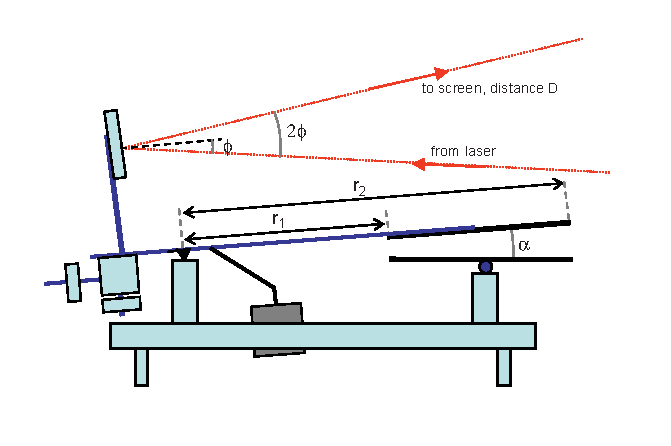
\includegraphics[width=4in]{coulbal.eps}
\caption{\label{fig:coulbal}
Sketch of the Coulomb balance used to measure electrostatic forces between
two plates.  A charge difference is placed on the two plates by connecting
a high-voltage source across them, not shown in the figure.  Masses are
placed in the center of the upper plate when no voltage is applied in order
to determine the gravitational force that is equivalent to the electrostatic
force at a given potential difference.  The displacement of the balance is
measured by monitoring displacements of the light spot on a vertical screen
located a distance $D$ from the mirror.  The screen is to the right, outside
the view shown in the figure.
}
\end{figure}

\begin{figure}
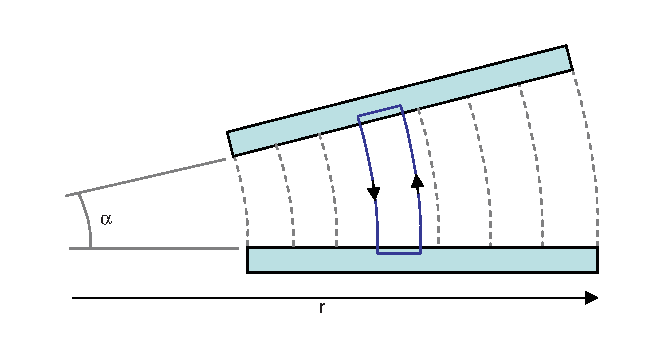
\includegraphics[width=4in]{efield.eps}
\caption{\label{fig:efield}
Diagram used to analyze the electric field pattern produced when two charged
conducting plates are supported next to each other in the geometry of the
Coulomb balance.  The dashed lines represent the electric field between the
plates.  The closed path in the illustration is used in the text to derive
an expression for the electric field between the plates as a function of
the radial distance $r$.
}
\end{figure}

\section{The Coulomb balance}

The Coulomb balance is a mechanical device that is used to measure the
magnitude of electrostatic attraction between two oppositely charged
bodies.  A side view of the apparatus is shown in Fig.~\ref{fig:coulbal},
showing the principal parts.  When a voltage source is connected between
the upper and lower arms of the balance, an electric field is set up between
the two plates, as illustrated in Fig.~\ref{fig:efield}.  Note that the
plates are only parallel when they are in contact, which cannot be the
case when they are charged.  When they are separated by an angle $\alpha$,
the two plates are no longer parallel, and so the field between them is
not uniform, but varies with radial distance $\alpha$.  For small values
of $\alpha$, the electric field lines follow a circular pattern with the
pivot point as its center, as shown in the figure, and distortions from
this pattern are confined to small regions near the edges.  These
distortions, which are sometimes called {\em edge effects} are ignored
in this treatment.

To derive how the electric field intensity varies with $r$, consider the
closed path shown in the middle of Fig.~\ref{fig:efield}.  Electrostatic forces
are conservative, so the total work one does in transporting a test charge
$q$ around this closed path must be zero.  The line segments at the top and
bottom of the loop involve no work because they are inside the conductor,
where the electric field is zero.  The inner arc-shaped path within the gap
contributes work $qE(r_i)r_i\alpha$, while the outer path contributes
$qE(r_o)r_o\alpha$, if the radii of the two arcs are $r_i$ and $r_o$,
respectively.  These two must sum to zero, leading to the result that
$r_iE(r_i)=r_oE(r_o)$.  Since this must hold for any values of $r_i$ and
$r_o$, it follows that $rE(r)=constant$, or
\begin{equation}
E(r)=\frac{U_0}{r}
\label{eq:Eofr}
\end{equation}
where $U_0$ is a constant yet to be determined.  To determine it,
consider the work done to carry a test charge $q$ along just one of
the arc-shaped paths between the two plates, whose absolute value is
$q\alpha rE(r)=q\alpha U_0$.  This value divided by $q$ is the
electric potential between the two plates, which is set by the voltage
$V$ coming from the external source.  Therefore $U_0=V/\alpha$.

Gauss's law requires
that the field $E$ above a conducting surface with local areal charge
density $\sigma$ is
\begin{equation}
E=\frac{\sigma}{\epsilon_0}
\end{equation}
which implies that $\sigma$ also varies like $1/r$ across the surface
of the plates.  Because the balance is only free to move rotationally,
the balance of forces must be computed as a sum of torques that add to
zero under conditions of equilibrium.

The torque coming from electrostatic attraction is computed in the
following way.  Consider the plates as having a width $W$ along the
rotation axis, and inner and outer radii $r_1$ and $r_2$ as shown
in Fig.~\ref{fig:coulbal}.  Break up the area of the upper plate into
small stripes of length $W$ and radial width $dr$.  The electrostatic
force on this stripe is proportional to the charge on this stripe times
the electric field $E(r)$.  Actually it is only half that value, because
the charges on the surface of the conductor are, roughly speaking, half
inside the conductor (where the field is zero) and half outside the
conductor (where the field is $E(r)$).  The total torque from electrostatic
forces is the sum of the forces on all of these stripes, multiplied by
their lever arms $r$.  Reducing this to an integral,
\begin{eqnarray}
\tau &=& -\frac{1}{2}\int_{r_1}^{r_2}{r\frac{U_0}{r}\sigma W\,dr} \nonumber\\
&=& -\frac{1}{2}\int_{r_1}^{r_2}{r\left(\frac{U_0}{r}\right)^2\epsilon_0 W\,dr} \nonumber\\
&=& -\frac{WV^2\epsilon_0}{2\alpha^2}\ln{\frac{r_2}{r_1}}
\label{eq:tauint}
\end{eqnarray}
In the experiment, the electrostatic torque is measured by comparing it
to the torque produced by the gravitational force acting on a known
mass $m$, which is treated as a point mass placed on the upper plate
at a distance $r_0$ from the rotation axis.  Setting these two torques
equal,
\begin{equation}
-mgr_0=-\frac{WV^2\epsilon_0}{2\alpha^2}\ln\left(\frac{r_2}{r_1}\right)
\end{equation}
which leads to the final result, in which the electrostatic constant
$\epsilon_0$ is computed in terms of known or measured quantities.
\begin{equation}
\epsilon_0 = \frac{2mg\alpha^2r_0}{WV^2\ln{r_2/r_1}}
\label{eq:epsilon0}
\end{equation}

\begin{figure}
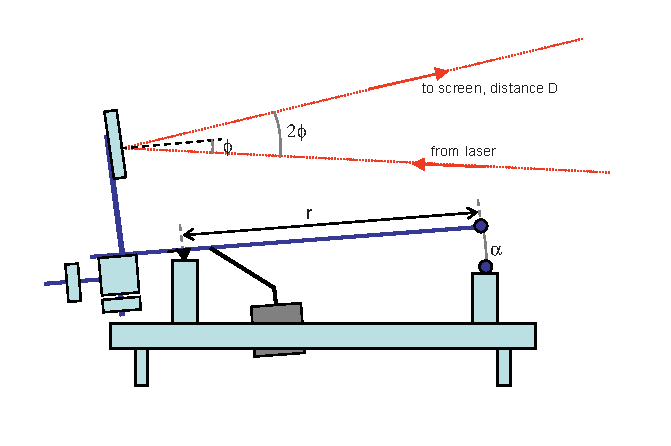
\includegraphics[width=4in]{curbal.eps}
\caption{\label{fig:curbal}
Sketch of the current balance used to measure magnetic forces between
two parallel wires.  An alternating current (in and out of the page in
the figure) is passed through the two wires
whose circular cross sections are visible to the right in the figure.  The
currents are in opposite directions, creating a repulsive force between the
two wires.  The force is compensated by adding weights to a small tray on
the upper wire, until the magnetic and gravitational forces cancel.
The displacement of the balance is
measured by monitoring displacements of the light spot on a vertical screen
located a distance $D$ from the mirror.  The screen is to the right, outside
the view shown in the figure.
}
\end{figure}

\begin{figure}
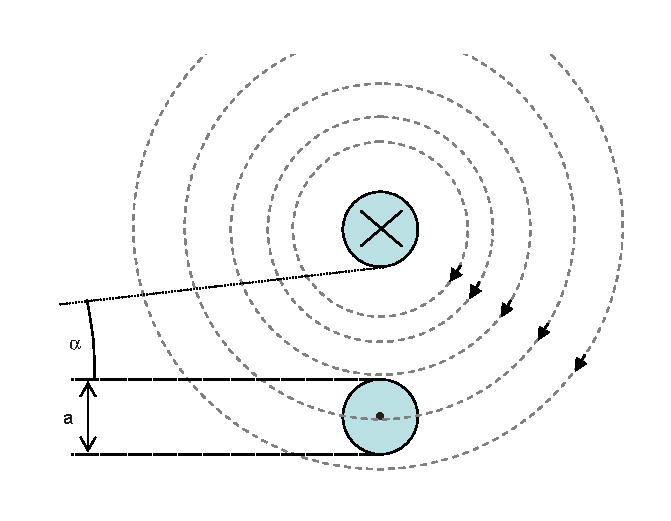
\includegraphics[width=4in]{bfield.eps}
\caption{\label{fig:bfield}
Diagram used to analyze the magnetic field pattern produced by the current
flowing in the upper wire.  The force on the lower wire is computed as the
action of this field on the current flowing in the lower wire, which is
assumed to be uniformly distributed across its cross section.
}
\end{figure}

\section{The current balance}

The current balance is very similar in its design to the Coulomb balance
described above, except that what is measured instead of the electrostatic
force is the magnetic force between two current-carrying wires.  A side
view of the apparatus is shown in Fig.~\ref{fig:curbal}.
When a current source is connected to the two ends of the conducting wires,
shown extending into the page in the figure, a magnetic field is set up
in the region around the wires, as illustrated in Fig.~\ref{fig:bfield}.
The magnetic field lines generated by the current flowing in the upper
wire follow a circular pattern around the axis of that wire, which extends
into the interior of the lower wire, where a current is present that flows
in the opposite direction.  This pattern is only exact for a wire of
infinite length. Distortions from this pattern are present near the
ends of the wires where the current changes direction.  These distortions,
which are sometimes called {\em end effects} are ignored in this treatment.

Because of the finite resistivity of the conductor, the current tends to
distribute itself uniformly across the cross sectional area of the wire.
This produces a magnetic field pattern that consists of circles centered
on the wire axis, as shown in Fig.~\ref{fig:bfield}.  Ampere's law gives
the magnitude of the magnetic field as a function of the distance $x$
from the center of the upper wire.
\begin{equation}
B(x)=\frac{\mu_0I}{2\pi x}
\end{equation}
To compute the net magnetic force between the two wires, consider first
the case where the wire diameter $a$ is negligible.  In that limit, the
current in the lower wire samples the magnetic field from the upper wire
at a single point a distance $x=\alpha r$ from the upper wire, leading to
the following expression for the repulsive force in the case of two
currents of the same magnitude $I$ and opposite direction flowing in
the two wires,
\begin{equation}
\tau=rBIL=\frac{\mu_0I^2L}{2\pi\alpha}
\label{eq:tauwitha0}
\end{equation}
where $L$ is the length of the parallel section of the two wires.

In this experiment, the approximation of negligible wire diameter $a$
is rather poor because one works with separations distances $r\alpha$
that are only one order of magnitude larger.  Because of this, some
attention must be given to the corrections to Eq.~\ref{eq:tauwitha0}
that occur with a non-zero value of $a$.  There are two independent
effects to be considered.  The first is that the distance between the
wires can no longer be taken to be $\alpha r$, but instead should be
the distance between the centers of the wires, which is $\alpha r+a$.
The second effect comes from the fact that the magnetic field from the
upper wire is not constant across the area of the lower wire, but is
strongest near the upper surface where it is closest to the upper wire,
and weakest near the bottom.  To take this into account, consider the
current flowing in the lower wire to be composed a circular bundle of
many tiny wires, each carrying a portion of the total current that is
proportional to its cross sectional area.  In the limit of many such
wires, the total force becomes an integral over the area of the lower
wire,
\begin{equation}
F= L\int_0^{a/2}y\,dy \int_0^{2\pi}d\phi B(x) j(y)
\end{equation}
where $x$ represents the distance of a point from the center of the
upper wire, $y$ is the distance of the same point from the center of
the lower wire, $\phi$ is the azimuthal angle of that point with
respect to the center of the lower wire, and $j(y)$ is the current
per unit area flowing on the lower wire, here assumed to be constant.

Since the integral is over $y\,dy\,d\phi$, we need to find how $B(x)$
depends on $y$ and $\phi$.  Using the law of cosines, this relationship is
\begin{equation}
x=\sqrt{x_0^2+y^2+2x_0y\cos{\phi}}
\end{equation}
leading to the result for the total force
\begin{equation}
F= \frac{\mu_0ILj}{2\pi}\int_0^{a/2}y\,dy \int_0^{2\pi}d\phi
\frac{1}{\sqrt{{x_0^2+y^2+2x_0y\cos{\phi}}}}
\end{equation}
where $x_0=\alpha r+a$ is the distance between the centers of the two wires.
This integral is very difficult to compute exactly, but a good approximation
can be obtained by noticing that the constant $x_0$ is about an order of
magnitude larger than $y$, so one can expand the integrand in powers of
$y/x_0$.  The first few terms in the Taylor series are
\begin{equation}
({x_0^2+y^2+2x_0y\cos{\phi}})^{-\frac{1}{2}} =
\frac{1}{x_0}\left[1
- \frac{y}{x_0}\cos{\phi}
-\left(\frac{1}{2}-\frac{3\cos^2{\phi}}{2}\right)\frac{y^2}{x_0^2}
+\left(\frac{3\cos{\phi}}{2}-\frac{5\cos^3{\phi}}{2}\right)\frac{y^3}{x_0^3}
+ {\cal O}\left(\frac{y}{x_0}\right)^4\right]
\end{equation}
Keeping only the first non-zero correction in $y/x_0$ leads to
\begin{equation}
F= \frac{\mu_0ILj}{2\pi x_0}\int_0^{a/2}y\,dy \int_0^{2\pi}d\phi
\,\left[1-
\left(\frac{1}{2}-\frac{3\cos^2{\phi}}{2}\right)\frac{y^2}{x_0^2}
+{\cal O}\left(\frac{y^4}{x_0^4}\right)\right]
\end{equation}
This integral is easy to evaluate, leading to
\begin{equation}
F = \frac{\mu_0LI^2}{2\pi x_0}\left[1+\frac{a^2}{32x_0^2}
+ {\cal O}\left(\frac{a}{x_0}\right)^4\right]
\label{eq:Fofa}
\end{equation}
Equating the torque from this magnetic force to the weight of a known
mass $m$ leads to an expression for the magnetic permeability constant
in terms of known or measured quantities.
\begin{equation}
\mu_0=\frac{64\pi x_0^3 mg}{LI^2(32x_0^2+a^2)}
\label{eq:mu0}
\end{equation}

\section{Experimental Procedure}

\begin{figure}
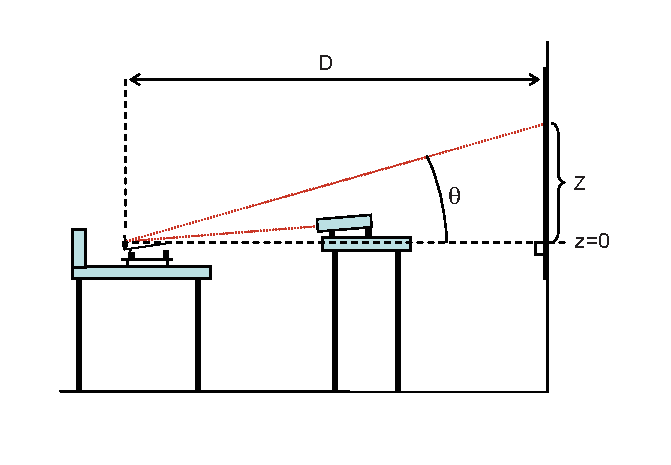
\includegraphics[width=4in]{distances.eps}
\caption{\label{fig:distances}
Diagram of the scheme used to precisely measure the angular displacement
of the balances used for this experiment.  Changes in the angle $\theta$ of
the reflected laser beam with respect to the horizontal are determined by
measuring the height $z$ of the beam spot on the viewing screen shown by 
the heavy vertical bar at the right side of the figure.
}
\end{figure}

The following initial set-up steps apply to either  the Coulomb balance
or the current balance.  The upper arm of the balance sits on two knife
edges which rest on the flat surfaces of two posts near the rear corners
of the base plate.  The balance is a delicate instrument and should be
handled carefully.  Particularly sensitive to damage are the two
knife edge suspension points and the surfaces upon which they
rest. The upper balance assembly can be raised off of the knife
edges by a lift mechanism.  The balance should be lifted off the
knife edges any time it is not in use.

Attached to the upper arm and hanging under it is
a vertical metal plate.  When the upper arm is properly aligned, this
plate should pass through a slot in the base plate.  Mounted in the base
plate on either side of the slot are magnets which induce a damping force
on the plate whenever it moves up or down inside the slot.  When everything
is properly aligned, the upper arm should be free to oscillate with an
amplitude of several degrees without the damping plate hitting anything or
scraping on the sides of the slot.  The oscillations should damp away with
a time constant between 5 and 10 seconds.  Make sure that the base plate
is resting on a firm level surface, and that it does not rock on its
supporting feet.  

There are two adjustable knobs on the back side of the upper arm of the
balance.  The one that extends horizontally out the back is used to set
the equilibrium position of the balance.  Adjust it by rotating it in one
direction or the other, until the equilibrium position of the balance is
found with the electrodes a few mm apart.  You may need to adjust this
later on during the measurements to find an optimal setting.  The knob
that is hanging under the upper arm is used to adjust the sensitivity
of the balance.  Raising it up makes the balance more sensitive, so that
its equilibrium position moves a larger amount in response to a given
torque.  Higher sensitivity also means that the balance is more susceptible
to vibrations and air currents, such that finding the equilibrium position
can be more difficult.  Finding an optimal compromise between stability
and sensitivity is one of the most important challenges in conducting
this experiment.

Throughout the measurement, it is important to minimize
any air currents in the vicinity of the balance.  This is true for both
measurements, but the Coulomb balance is particularly sensitive because
of the large area of the plates.  People in the room should minimize their
movements while measurements are being taken, so that the balance can
reach equilibrium for a long enough period for measurements to be taken.

Displacements of the balance will be measured using a laser beam reflecting
off the mirror on the upper arm of the balance onto a viewing screen some
distance away, as shown in Fig.~\ref{fig:distances}.
The viewing screen should be mounted on a fixed vertical
surface.  A white board mounted on the wall is a good choice, allowing
displacements to be recorded using a marker.  Mount the mirror in the space
between the screen and the balance and align it so that the beam is
centered on the mirror.  The incident beam direction should be pointing
slightly downward, as shown in the figure, so that the reflected spot
remains within the range of the white board.  Check that the reflected
beam spot on the viewing screen is visible without obstruction through
the full range of motion of the upper balance arm.  Check that the plane
swept out by the reflected laser beam, as the upper arm of the balance
moves through its range of motion, intersects the screen at right angles
to within a few degrees.

Carefully mark the point labeled $z=0$ on the screen.  This will serve as
the origin for all measurements of $z$ throughout the experiment.  Measure
and record the distance $D$, together with its error.  Once $D$ has been
measured and the point $z=0$ marked on the screen, make sure the laser and
balance are not moved.  If either one is disturbed after this, stop the
measurements and go back and start from the beginning again.

\subsection{Coulomb balance procedure}

Carry out the above steps to set up the balance for measurements.  Make
sure that the orientation of the lower plate is such that the two plates
are parallel and touching everywhere when they come together.  Align the
upper arm on its mounts so that the edges and corners of the upper and lower
plates line up as exactly as possible.  Measure the width $W$ of the upper
and lower plates using a vernier caliper.  Take the average of your two
measurements as the value for $W$, and record your measurement error.
Measure the length of the two plates, and record their average values as
$H$, together with its measurement error. On the upper plate, measure the
distance $r_1$, which is the radial distance between the rocking axis defined
by the knife edges and the inner edge of the plate, as shown in 
Fig.~\ref{fig:coulbal}.  The value of $r_2$ is obtained as $r_1+H$.
On the top of the upper plate is a cross-hair marking the spot where you
will place weights during the measurement.  Measure the distance $H_2$
from the cross hair to the center of the inner edge of the plate, and
record its value and error.  Confirm that $H_2 = H/2$ within measurement
error.

Prepare several small weights with masses between 20 and 200 mg to be used
during the measurement.  One convenient way to do this is to cut out strips
of office paper with different areas.  Before cutting the paper, measure the
mass per unit area of the paper by weighing an entire sheet and measuring its
area.  Be aware that the density of office paper can vary from one package to
the next, and is highly sensitive to the ambient humidity in the area where
it is stored.  If you chose to weigh more than one sheet at a time for
increased accuracy, make sure that all of the sheets came from the same
package and were stored together during the time since the package was
opened.  Determine the masses of your paper weights by measuring their
dimensions as you cut them out, together with your measurement errors.
Make sure that the equilibrium position of the unweighted balance is set
high enough that the plates do not come into contact when the heaviest of
your masses is placed in the center of the upper plate, but that they do
come together when a penny is used.

Because the electric force measured in the Coulomb balance is attractive
and increases with decreasing separation between the plates, special
restrictions must hold in order to achieve stable equilibrium.  A detailed
analysis of these conditions is presented in App.~\ref{app:stability}.
In summary, stable equilibrium with high voltage present on the plates
can only be achieved if the separation angle $\alpha$ is greater than
$(2/3)\alpha_0$, where $\alpha_0$ is the equilibrium separation angle 
of the unweighted plates when the voltage is zero.  To minimize edge
effects, you should make sure that the equilibrium settings with the
weights present are in the range where the plates are 5-15~mm
apart.  Putting all of this together, set the unweighted equilibrium
point such that the plates are about 10-20~mm apart.  Adjust the sensitivity
so that adding the lightest weights produces a significant displacement
from $\alpha_0$, but not sinking past $(2/3)\alpha_0$.  As you increase
the weight added to the upper plate, watch that the displacement does
not push the balance below $(2/3)\alpha_0$.  When it does,
stop and switch over to measuring in high-voltage mode (see below), then
come back later and decrease the sensitivity of the balance in order to
do the heavier weights.  Remember that it is a waste of your
time to measure displacements past $(2/3)\alpha_0$ because, if you do,
you will not be able to achieve stability at an equivalent displacement
using electric forces later.  Stability under electric forces is only
possible under the condition that $(2/3)\alpha_0<\alpha<\alpha_0$.

Place the penny on the upper plate and record the displacement of the beam
spot on the viewing screen as $m=\infty$.  Take off the penny and measure the
unweighted equilibrium displacement of the spot on the screen, marking it
as $m=0$ on the screen.  Record the $z$ positions and errors $\Delta z$ for
these two limiting mass values.  The $z$ positions for all intermediate
masses between 0 and $\infty$ will lie between these two limits.  Using a
meter stick, mark the point that is
2/3 the way from $m=\infty$ to the $m=0$ mark.  In all of the subsequent
measurements in this run, you should make sure that you do not go below
this line.  One by one, starting with the smallest mass, place each one
on the cross-hairs in the middle of the upper plate and record the
values of $z$ and errors $\Delta z$ for each.  Be careful in placing the
weights on the plate that you do not knock or disturb its alignment in any
way.  If you are using weights cut from a sheet of paper, fold the paper
so that it can be easily centered on the cross hairs and picked up without
touching the apparatus, or use tweezers to place and remove them.

Turn on the high-voltage supply and test it using a volt meter and a
high-voltage probe that has been approved by your TA for this purpose.
After confirming that the supply is working, set the output voltage to
zero and turn off the supply.  Remove all of the masses from the upper
plate of the balance and connect the high-voltage supply to its two
electrical terminals.  Unless you know that the power supply is internally
protected against shorts, a large resistor (10 M$\Omega$) should be
used between the supply and the terminal on the high-voltage side to prevent
damage to the supply, should an arc accidentally occur between the two plates.
{\em This resistor is does not make the apparatus safe to touch when the high
voltage is present!}  Establish and respect a safety zone of 20-30 cm in
all directions around the apparatus while the high-voltage supply is
connected.  Besides body parts, this also includes all clothing and any
items such as notebooks, pens, or any electronics that is not required for
operating the balance.  A good rule is to announce ``voltage on'' each time
that high voltage is present on the balance, and ``voltage off'' each time
it is removed, so that everyone present in the room is aware of conditions on
the bench.

Turn on the high-voltage supply and slowly ramp up the voltage, watching
the spot on the screen for the first sign of a shift in the equilibrium
position.  This should occur within the first 200 volts.  Now increase the
voltage more slowly, waiting between steps for the balance to find its
new equilibrium, until you reach the displacement that you recorded for
the lightest weight.  Using the high-voltage probe, record the voltage
reading that gives the best match to that
displacement, then vary it above and below this point to find your
measurement error on $V$.  Continue increasing the voltage until you find
values for $V$ and $\Delta V$ for each of the heavier masses.

If it does happen that you increase $V$ high enough that the plates dip
below the $(2/3) \alpha_0$ point, they will eventually come together and
touch, creating a spark.  This is not a disaster, but requires prompt action.
Turn off the high-voltage supply using the on/off switch, then turn the
control knob down to zero.  The balance usually swings strongly after 
sparking, so wait for it to settle down again, then turn the supply on
again and ramp the voltage back up again.  If air currents are responsible
for the oscillations that caused the spark, try to reduce them before
continuing your measurements.  There is a practical minimum distance for
the separation between the plates close to 1~mm, below which it is
practically very difficult to make a measurement without sparking.  If
you find that your heaviest mass results in a plate spacing that is too
small, you may need to adjust the equilibrium balance position to a higher
setting and repeat the measurement.

Turn off the high-voltage supply and disconnect it from the balance.
Use a lead to short the two arms of the balance together, then announce
``voltage off'', before touching the apparatus with your hands.  You
will need to remember to remove the shorting cable before turning on
the voltage again later.
Increase the equilibrium position by adjusting the knob on the back of
the upper plate, then repeat all of the above measurements a second time,
starting with a re-measurement of the $m=\infty$ point with the penny,
and the $m=0$ point without any weights present.  You will
find that with a higher equilibrium position, larger high voltage values
will be required to achieve a match with the displacement for a given
weight.  If this requires raising the high voltage higher than the supply
can safely provide, you may chose to create and substitute some new lighter
weights instead.  If you do this, keep in mind that the percent errors on
the paper masses will increase substantially for masses less than 10~mg.

\subsection{current balance procedure}

Carry out the steps outlined at the head of this section
to set up the balance for measurements.  Make
sure that the upper and lower wires of the current balance are straight
and parallel so that they are touching all along their length when the
two arms come together.  Align the upper arm on its mounts so that the
two wires are lined up as exactly as possible, when viewed from above.
Measure the length $L$ of the section of the two wires where they are
running parallel to each other.  Take the average of your two
measurements as the value for $L$, and record your measurement error.
On the upper arm, measure the distance $r$, which is the radial distance
between the rocking axis defined by the knife edges and the center of the
wire, as shown in Fig.~\ref{fig:curbal}.  Use a vernier caliper to measure
the diameters of the upper and lower wires.  Record the average value
as $a$, together with your measurement error.
On the top of the upper wire is a small tray where you will place weights
during the measurement.  Make sure that the center of the tray is aligned
with the center of the wire, so that a second measurement for $r$ is not
needed.

Prepare several small weights with masses between 20 and 200 mg to be used
during the measurement.  One convenient way to do this is to cut out strips
of office paper with different areas.  Before cutting the paper, measure the
mass per unit area of the paper by weighing an entire sheet and measuring its
area.  Be aware that the density of office paper can vary from one package to
the next, and is highly sensitive to the ambient humidity in the area where
it is stored.  If you chose to weigh more than one sheet at a time for
increased accuracy, make sure that all of the sheets came from the same
package and were stored together during the time since the package was
opened.  Determine the masses of your paper weights by measuring their
dimensions as you cut them out, together with your measurement errors.

Carefully place the penny in the tray on the upper wire, making sure that
the wires come into full contact when at rest.
Record the displacement of the beam spot on the viewing screen as 
$z=0$.  All other displacements will be measured
using this position as the origin.  Adjust the equilibrium position of
the balance so that it comes to rest with the wires several mm 
(less than 10) apart.  Adjust the sensitivity of the balance so that
there is little oscillation of the bars after a minute of settling time,
or at least that the center of the oscillations can be accurately 
determined.

The earth's magnetic field is sufficiently strong to produce forces that
can distort the results of this measurement, depending on how the balance
is oriented.  To avoid this complication, an alternating-current supply
is used.  An AC current supply capable of producing 20~A into a few Ohms
resistance can be built using a pair of Variacs and a step-down transformer.
Turn the power switches to off on both of the Variacs.
Connect the Variacs in series, and the output of the second one to the
primary winding of the transformer.  Connect the secondary winding of
the transformer to the two terminals of a current meter, making sure that
the meter is capable of at least 10~A.  Turn the first Variac to zero and
the second one to its maximum setting.  Plug the first Variac into a power
outlet and turn it on.  Slowly ramp up the current by turning up the
output of the first Variac, that was set to zero in a preceding step.
Watch the current meter as you ramp it up, and confirm that you can reach
10~A before going above half the maximum output on the first Variac.
Ramp the current back down to zero by lowering the output of the first
Variac.  The control on the first Variac is the current control knob for
the remainder of this experiment.

Disconnect the current meter from the transformer output, and in its place
connect the transformer to the terminals of the current balance.  Using a
heavy copper lead, connect the far terminal of the upper wire to the far
terminal of the lower wire.  This way, the currents through the two wires
are going in opposite directions in the straight parallel section.  The
current meter is not connected in series with the balance for this
measurement because it may be damaged by the currents as high as we
wish to use.  Instead, you will measure the current indirectly by measuring
the voltage drop along the heavy copper lead that conducts the current between
the upper and lower arms of the balance.  Disconnect the copper lead from
the apparatus and measure its resistance.  This resistance will increase
as the wire heats up under heavy current load, so you will need to measure
it several times throughout the experiment.  The resistance is small, so
you need to measure the resistance of the voltmeter leads and subtract them
away to get an accurate value.  Measure this resistance with a second
ohmmeter and a different pair of leads to obtain an estimate of your
measurement error.  Then reconnect the copper leads to the balance, and
place a voltmeter across its two ends to record the voltage drop.  Make
sure the voltmeter is in AC mode.

Because the current balance is arranged to measure repulsive rather than
attractive forces, there are no restrictive conditions for stable
equilibrium with the current balance like there were for the Coulomb
balance.  The only restriction on the permissible range of $\alpha$
is that the two wires should be more than 2 diameters apart at equilibrium,
otherwise higher-order terms that have been dropped in Eq.~\ref{eq:Fofa}
might contribute significantly and throw off the analysis.

With no weights in the tray and no current flowing in the wires, measure
the equilibrium position $z_0$ of the balance.  Now place the smallest mass
into the weight tray.  This should cause the upper arm of the balance to
move downward.  Slowly ramp up the current through the wires until the
displacement moves back to its original position $z_0$.  Record the value
of the voltage drop across the copper lead as an indicator of the current
in the wire.  Adjust the current above and below the central value and
obtain an estimate of the measurement error on the current needed to
balance the weight of the mass.  Turn off the current, quickly remove
the copper lead, and measure its resistance.  At currents of 1-2~A there
should not be much change in the resistance, but at higher currents there
may be a substantial increase due to heating.  This is why the measurement
should take place promptly after turning off the current source, before the
wire has had a change to cool off.

At this point you should also check for
hot spots along the wire.  A defective lead may develop hot spots, often
near the end terminals, that can lead to melting of the insulation.  Any
time you smell a scent of burning you should turn off the current source
immediately and investigate the cause of the smell.  In no case should
you increase the current above 20~A.

Turn off the current supply and disconnect it from the balance.
Increase the equilibrium position by adjusting the knob on the back of
the upper plate, then repeat all of the above measurements a second time,
starting with a re-measurement of the $z=0$ point with the penny.  You will
find that with a higher equilibrium position, larger current values
will be required to achieve equilibrium given weight.  If this requires
raising the current higher than 20~A, 
you may chose to create and substitute some new lighter
weights instead.  If you do this, keep in mind that the percent errors on
the paper masses will increase substantially for masses less than 10~mg.

\section{Data Analysis}

For the Coulomb balance, Eq.~\ref{eq:epsilon0} predicts that a plot of
$(V/\alpha)^2$ vs.\ $m$ will yield a straight line with a zero y-intercept.
Experimental values for $\alpha$ are obtained using the relations,
\begin{eqnarray}
\theta &=& \arctan\left(\frac{z}{D}\right) \nonumber \\
\alpha &=& \frac{\theta-\theta_{\infty}}{2}
\label{eq:alpha}
\end{eqnarray}
where $z$ is the spot displacement on the viewing screen relative to the
point $z=0$ shown in Fig.~\ref{fig:distances}, and $\theta_{\infty}$ is
the value of $\theta$ at the $m=\infty$ point, where $\alpha$ is defined
to be zero.  Fit your data for $(V/\alpha)^2$ vs.\ $m$
to a straight line using a least-squares fit.  Be sure to propagate the
errors from $V$ and $\alpha$ into total errors for the points on the $y$
axis of the fit plot.  Compute the contribution to the errors 
coming from the uncertainties on the $m$ values as $\Delta m$ 
multiplied by the slope of the best-fit line.  These should be added in
quadrature to the errors coming from $V$ and $\alpha$ in computing the
total error $\Delta y$ for each data point.  Verify that the y-intercept
of this line is zero within the error.  Use the slope of this line and
its error, together with the values of the other parameters in
Eq.~\ref{eq:epsilon0} and their errors, to extract a measured value for
$\epsilon_0$ and its uncertainty.  Compare this result to the accepted
value for $\epsilon_0$.

For the current balance, Eq.~\ref{eq:mu0} predicts a linear relationship
between $I^2$ and $m$ for a given equilibrium displacement $\alpha$.
Experimental values for $\alpha$ are obtained using Eq.~\ref{eq:alpha}.
Fit your data for $I^2$ vs.\ $m$ to a straight line using a least-squares
fit.  Be sure to propagate the errors from $I$ into errors on $I^2$ to
obtain errors for the points on the $y$ axis of the fit plot.  Compute
the contribution to the errors coming from the uncertainties on the $m$
values as $\Delta m$ multiplied by the slope of the best-fit line.
These should be added in quadrature to the errors coming from $I$ in
computing the total error $\Delta y$ for each data point.  Verify that
the y-intercept of this line is zero within the error.  Use the slope of
this line and its error, together with the values of the other parameters in
Eq.~\ref{eq:mu0} and their errors, to extract a measured value for
$\mu_0$.  Compare this result to the accepted value for $\mu_0$.

One of the triumphs of Maxwell's classical theory of electromagnetism
is its prediction for the speed of light waves in vacuum.  If light is
an electromagnetic wave then Maxwell's equations predict that it should
travel at a unique speed $c$ in vacuum, regardless of its wavelength.
This value is
\begin{equation}
c=\sqrt{\frac{1}{\epsilon_0\mu_0}}
\label{eq:c}
\end{equation}
Use your measured values for $\epsilon_0$ and $\mu_0$ to estimate the
speed of light in vacuum, and your uncertainty on this value.
Compare your estimate with the published value of $c$.

  The physical constants $\epsilon_0$ and
$\mu_0$ actually apply only to measurements made in vacuum, whereas
your measurements are made in air.  Use the published value of the index
of refraction of light in air to argue that corrections for the presence
of air in this experiment are expected to be much smaller than the
experimental uncertainties coming from the measurement.

\begin{acknowledgments}
This document was written by Prof. Richard Jones, based on an earlier
write-up by Prof. Ed Eyler and on information contained in the User's
Manuals for the Coulomb balance and the current balance issued by their
manufacturer, Sargent-Welch Scientific Co., 7300 N. Linder Ave., Skokie,
Ill. 60076.
\end{acknowledgments}

%% Create the reference section using BibTeX:
%\bibliography{revtex4}

%\begin{thebibliography}{9}
%
%\bibitem{Tznpo71}
%Lfjui S. Tznpo,
%\emph{Nfdibojdt},
%Beejtpo-Xftmfz, Sfbejoh NB,
%3se fe. (1971) pp. 214-215.
%
%\bibitem{Lmfqqofs73}
%E. Lmfqqofs boe S.K. Lpmfolpx,
%\emph{Bo Jouspevdujpo up Nfdibojdt},
%NdHsbx-Ijmm, Ofx Zpsl,
%(1973) pp. 257-257.
%
%\bibitem{Nbsjpo95}
%K.C. Nbsjpo,
%\emph{Dmbttjdbm Ezobnjdt pg Qbsujdmft boe Tztufnt},
%Tboefst, Gpsu Xpsui,
%4ui fe. (1995) p. 455.
%
%\bibitem{Ifjtlbofo67}
%X.B. Ifjtlbofo, boe I. Npsjua,
%\emph{Qiztjdbm Hfpeftz},
%X.I. Gsffnbo, Tbo Gsbodjtdp
%(1967).
%
%\end{thebibliography}

\newpage

\appendix
\section{Stability of the Coulomb balance}
\label{app:stability}
\setcounter{figure}{0}
\renewcommand*\thefigure{\Alph{section}.\arabic{figure}}

The conditions for equilibrium of a balance are that the center of gravity
is directly under the pivot point.  Angular displacements in either direction
from this equilibrium result in a restoring torque that tends to bring it
back toward the equilibrium angle, here denoted $\alpha_0$.  The potential
$U(\alpha)$ corresponding to this torque is
\begin{equation}
U_0(\alpha) = \frac{1}{2}k(\alpha-\alpha_0)^2
\label{eq:U0}
\end{equation}
where $k$ is the Hooke's Law coefficient of the restoring force.  The
zero subscript on $U_0$ is there because this potential only holds when
$V=0$.  When $V$ differs from zero, there is an additional torque due to
electric forces that is given by Eq.~\ref{eq:tauint}.  Including this
force leads to the combined potential 
\begin{equation}
U(\alpha) = \frac{1}{2}k(\alpha-\alpha_0)^2 - \frac{AV^2}{\alpha}
\label{eq:UofV}
\end{equation}
where the constant $A=(W\epsilon_0/2)\ln{r_2/r_1}$.  The overall shape
of the potential is governed by the size of the voltage $V$ that appears
in the second term in Eq.~\ref{eq:UofV}.  For small values of $V$, the
shape of the potential is like the solid curve shown in the first panel
of Fig.~\ref{fig:upalpha}.  This potential exhibits a stable equilibrium
about a position that is close to $\alpha_0$ but somewhat less.  The dashed
curve shows what happens to the shape of the potential curve for larger
values of $V$.  Here the local minimum in the potential has disappeared
and there is no longer a stable equilibrium anywhere except at $\alpha=0$.

\begin{figure}
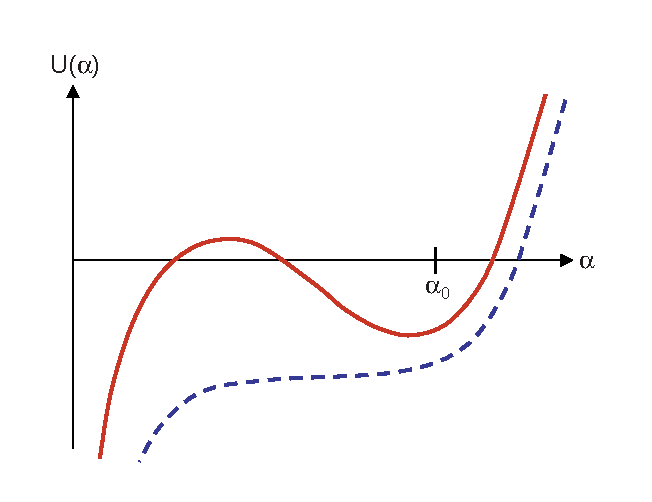
\includegraphics[width=3in]{ualpha.eps}
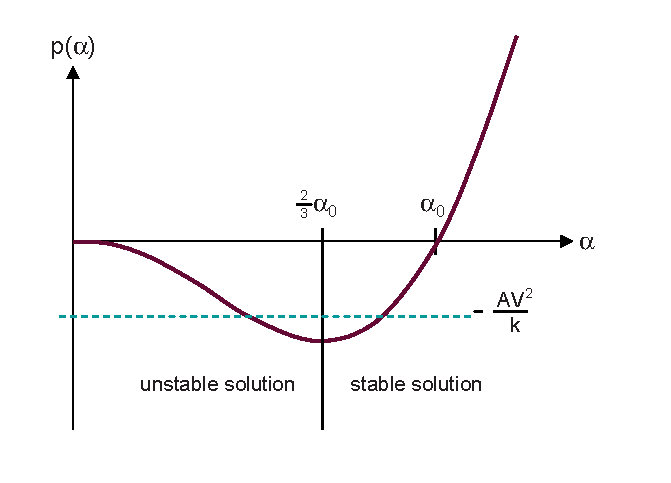
\includegraphics[width=3in]{palpha.eps}
\caption{\label{fig:upalpha}
Illustration of the conditions for stability in the Coulomb balance.
The first panel shows the potential energy of the balance as a function
of displacement $\alpha$ for a small value of the high voltage $V$ (solid
red curve) and a large value of $V$ (dashed line).  The second panel
illustrates the behavior of the function $p(\alpha)$ defined in
Eq.~\ref{eq:palpha} and the correspondence of its two positive roots to
stable and unstable equilibrium solutions.
}
\end{figure}

To find out under what conditions the stable equilibrium exists, one
solves for the roots of the first derivative of the potential.  If there
are two positive roots then the lesser of the two corresponds to the 
unstable equilibrium at the local maximum in the potential, and the
greater root corresponds to the stable equilibrium at the local minimum.
If there is no positive root then there is no stable equilibrium.  The
zeroes of the function $dU/d\alpha$ satisfy the equation
\begin{equation}
\alpha^2(\alpha-\alpha_0) = -\frac{AV^2}{k}
\label{eq:palpha}
\end{equation}
Calling the left-hand side of Eq.~\ref{eq:palpha} $p(\alpha)$, the roots
of this equation are illustrated in the second panel of Fig.~\ref{fig:upalpha}.
The minimum in the function $p(\alpha)$ appears at $\alpha=(2/3)\alpha_0$.
If $V$ is not too large, there are two positive roots, corresponding to the
unstable and stable equilibria of the potential, as shown in the figure.
If $V$ is increased further, the two roots eventually meet at 
$(2/3)\alpha_0$, and then disappear.

This analysis leads to the following simple conclusions. If an equilibrium
exists at all with $V>0$, then it exists in the window between $(2/3)\alpha_0$
and $\alpha_0$.  Conversely, for any displacement $\alpha$ within this
window, it is possible to find a value of $V$ for which $\alpha$ represents
a stable equilibrium of the system.  For any displacement $\alpha$ outside
this window, it is impossible to find a value of $V$ for which $\alpha$
represents a stable equilibrium.

\end{document}
%%
%% ****** End of file template.aps ******
%
%
